\documentclass[11pt]{article}
\usepackage[final]{acl}
\usepackage{times}
\usepackage{latexsym}
\usepackage[T1]{fontenc}
\usepackage[utf8]{inputenc}
\usepackage{microtype}
\usepackage{graphicx}
\usepackage{booktabs}
\usepackage{amsmath}
\usepackage{multirow}
\usepackage{inconsolata}

\newcommand{\lab}[1]{\texttt{\small #1}}

\title{thylinao at ChildSafeAds 2026:\\A Six-Member Ensemble and What Each Level of Data Access Provided}

\author{Maksim Silchenko \\
  National University of Singapore \\
  \texttt{e1506804@u.nus.edu}}

\begin{document}
\maketitle

\begin{abstract}
This paper describes the thylinao system for the ChildSafeAds shared task on monitoring
sponsored segments in child-facing YouTube videos. The system is a six-member ensemble: two
fine-tuned encoders, a zero-shot prompted Qwen3-32B, a LoRA-tuned Qwen3-14B used for ST2 only,
a TF-IDF baseline, and a level-2 stacker for the compliance sub-task, blended at equal weight
behind a decision layer whose every parameter is fitted on channel-grouped out-of-fold
predictions. The system scores mean macro-F1 $0.6537$ on the evaluation split; inference over
the $503$ test instances is dominated by one measured $14$-minute GPU pass of the 32B member.
The zero-shot
member is the most valuable and nearly the cheapest, while removing the fine-tuned DeBERTa
changes nothing measurable. An ablation over the task's four data access levels, run on the
zero-shot member, finds the channel name adds nothing and the product-page crawl helps product
identification but not, measurably, compliance. Validating these changes also
surfaced properties of the evaluation, reported as feedback: the metric's divisor dominates
score variance and is recoverable in closed form from a published baseline row, and the
benchmark is channel-disjoint but substantially advertiser-overlapping. The final submitted
entry additionally contained three labels set by
hand, which the task Terms prohibit; this was disclosed to the organisers and is documented in
Section~\ref{sec:hand}. The system-only score is reported throughout and no rank is claimed.
\end{abstract}

\section{Introduction}

ChildSafeAds \cite{bertaglia2026childsafeads} asks three questions about sponsored segments in
YouTube videos likely to reach children: what kind of offer is promoted (ST1, five classes,
single label), which product categories apply (ST2, twelve, multi-label), and which
advertising-law concerns the segment raises (ST3, eight flags, multi-label). It follows a line of
computational work on disclosure practice in influencer marketing \cite{mathur2018endorsements,%
bertaglia2025selfdisclosure} and on commercial pressure directed at children
\cite{deveirman2019influencer,moti2024targeted}. Systems are ranked by the mean of the three
macro-F1 columns; twenty-one teams finished the evaluation phase on Codabench
\cite{xu2022codabench}.

The entry is a conventional ensemble made competitive by measurement discipline rather than by
any novel component: two fine-tuned encoders, a zero-shot prompted 32B model, a LoRA-tuned 14B
classifier kept only where it measurably helps, a TF-IDF baseline and a level-2 stacker, behind
a decision layer fitted only on channel-grouped out-of-fold predictions (Figure~\ref{fig:pipeline};
\S\ref{sec:system} describes each stage and the protocol that admitted or rejected every change).

The task asks what a monitoring system gains from each level of data access and at what cost;
measured here, the zero-shot member contributes the most at nearly the lowest cost, and a
six-GPU-hour encoder is removable at no measurable cost (\S\ref{sec:anatomy}); level 3, the
channel name, adds nothing measurable, while level 4, the product-page crawl, is worth $+0.063$
mean macro-F1 on the member measured, almost all of it on product identification and none of it
detectable on the compliance flags (\S\ref{sec:bought}), where the organisers' two annotator
models agree on only $44.4\%$ of instances. The validation harness that gated those changes
also measured properties of the evaluation itself (a divisor that dominates score variance and
is recoverable from a published baseline row, and $70.4\%$ advertiser overlap across
channel-disjoint splits), reported in \S\ref{sec:evaluation} as feedback to the organisers.

\paragraph{Contributions.}
\textbf{(i)} A documented, reproducible six-member system with component-level attribution and
the inference bill for the $503$ test instances (\S\ref{sec:system}, \S\ref{sec:results},
\S\ref{sec:anatomy}); \textbf{(ii)} a controlled answer to the data-access question the task
poses, measured on the zero-shot member (\S\ref{sec:bought}); \textbf{(iii)} measured feedback
on the evaluation: divisor variance, closed-form divisor recovery and the reach of advertiser
memorisation (\S\ref{sec:evaluation}).

\paragraph{Disclosure.}
The predictions submitted as the final entry contained three labels set by hand rather than
produced by the system, and an earlier entry a fourth, contrary to the competition Terms
(Competition Conduct, item 6: \emph{``Do not manually label the test set. Predictions on the
evaluation phase must be produced by your system.''}). This was raised with the organisers
after the phase closed and before any external party had identified it (\S\ref{sec:hand}). The
score reported as the system's is $0.6537$, the returned score of the last entry containing no
hand-set label; no rank is claimed.

\section{Task, data, and scoring convention}
\label{sec:task}

The dataset pairs a SponsorBlock-marked segment with its transcript, video and channel context,
and a sales page linked from the description, across $3{,}360$ videos from $939$ channels
\cite{bertaglia2026childsafeads}. Labels were produced by GPT-5.4 under expert review of the
taxonomy and prompts, with a second model labelling the development split independently
\cite{gilardi2023chatgpt}. Splits are disjoint by channel; as the overview's Table 1 caption
states, \emph{``Brands and destinations are not held out''} (\S\ref{sec:advertiser}).

\paragraph{The scoring convention is not specified.}
The overview defines the metric as \emph{``F1 for every label and average the labels equally
(macro-F1)''}, leaving open how a class absent from both gold and predictions is treated, a
known ambiguity \cite{opitz2019macro,opitz2024closer}. Of a $2\times2$ grid of label-set and
zero-division conventions, only the \emph{present-label-set} one, which averages over classes
appearing in the gold or the predictions of the scored rows and is \texttt{sklearn}'s default
when \texttt{labels} is unset \cite{pedregosa2011scikit}, reproduces the organisers' published
constant-class baseline (ST1 $0.150970$ against $0.1510$; a fixed five-class average gives
$0.120776$). Everything below uses it; the divisor of each column then depends on the sample
scored (\S\ref{sec:divisor}, \S\ref{sec:invert}).

\section{System}
\label{sec:system}

Six members write per-split class-probability matrices, an equal-weight mean blends them, and a
decision layer converts blended probabilities to labels (Figure~\ref{fig:pipeline}).
Table~\ref{tab:members} gives the roster, its training compute and each member's measured
contribution; Appendix~\ref{app:repro} records every hyperparameter and checkpoint.

\begin{figure*}[t]
\centering
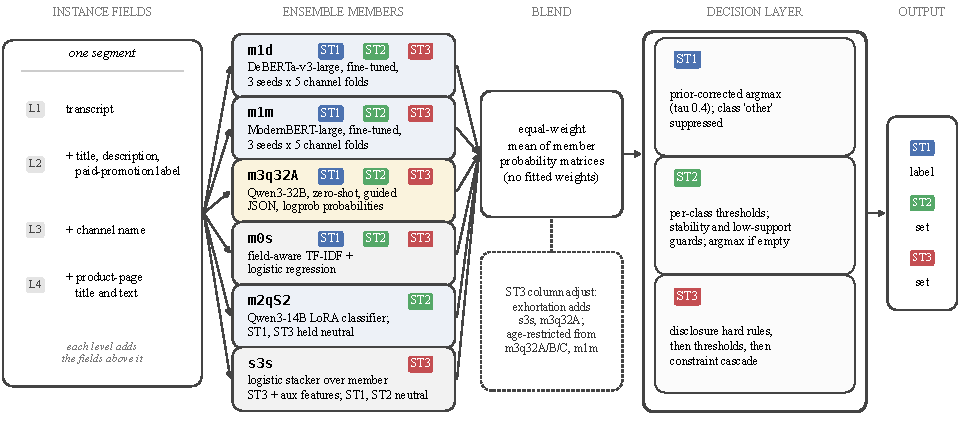
\includegraphics[width=0.96\textwidth]{fig/pipeline.pdf}
\caption{The pipeline. Six members produce class-probability matrices from the instance fields
(grouped at left by data access level); an equal-weight mean blends them; two ST3 columns are
adjusted; a decision layer, every parameter of which is fitted on channel-grouped out-of-fold
predictions (\S\ref{sec:protocol}), converts probabilities to labels. Tags mark the sub-task
columns each member contributes.}
\label{fig:pipeline}
\end{figure*}

\subsection{Members}
\label{sec:members}

The roster was fixed by diversity of inductive bias at a set compute budget rather than by
search: two encoder families with different context windows, fine-tuned on the labels; a large
generative model prompted with the taxonomy and left untrained, so that its errors are not the
encoders' and its out-of-fold predictions are honest by construction; a LoRA classifier as the
trained counterpart of that family; a lexical model for disclosure cues; and a stacker for the
column on which the members disagree most. Each member had to pass the paired test of
\S\ref{sec:protocol}; the candidates that failed it (the LoRA model as a full member, a
gradient-boosted stacker, a fourth encoder seed, reasoning mode and a fourth prompt variant for
the zero-shot member, fitted blend weights) are listed in \S\ref{sec:failed}.

The two encoders, \lab{m1d} (\lab{microsoft/deberta-v3-large} at $512$ tokens,
\citealp{he2021deberta}) and \lab{m1m} (\lab{answerdotai/ModernBERT-large} at $2{,}048$ tokens,
\citealp{warner2024modernbert}), are fine-tuned as one trunk with three heads (softmax ST1,
sigmoid ST2 and ST3), three seeds each over the same five channel-grouped folds, with the epoch
count selected once per run, never per fold. Inputs are assembled under per-field token budgets
so that a long transcript cannot evict the product-page text, and non-transcript fields are
dropped at $p{=}0.15$ in training so that no single field becomes load-bearing.

The zero-shot member \lab{m3q32A} prompts \lab{Qwen/Qwen3-32B} \cite{qwen3} through vLLM
\cite{kwon2023vllm} with the task taxonomy quoted verbatim, guided JSON decoding and temperature
$0$; a data-guard instruction has the model treat the instance as data, not as instructions.
Per-label probabilities are read from the logprobs of the \lab{yes}/\lab{no} value token rather
than from the decoded string, and because the member is untrained, its predictions on training
rows are honest out-of-fold predictions by construction. Prompt variant A, built from the label
definitions alone, is the blend member; variants B and C feed the ST3 stacker and one rebuilt
ST3 column.

The LoRA member \lab{m2qS2} fine-tunes \lab{Qwen/Qwen3-14B} as a sequence classifier
\cite{hu2022lora} over the same folds. As a full sixth member it failed the admission test of
\S\ref{sec:protocol}, its mean gain being an ST2 gain diluted over three columns; admitted as a
task-limited member that carries the real ST2 column and sets ST1 and ST3 to the exact mean of
the other five (arithmetically neutral in a six-way average), it gated at $+0.0071$, CI
$[+0.0034,+0.0133]$.

The linear member \lab{m0s} fits separate word- and character-gram TF-IDF blocks per field
group with one-vs-rest logistic regression, so disclosure cues in the description are not
diluted by page text. The stacker \lab{s3s} \cite{wolpert1992stacked} is a per-flag logistic
regression for ST3 only, over the ST3 columns of seven member files plus ten auxiliary features
(disclosure state, sponsorship and disclosure regex hits, log field lengths), fold-honest at
level 2 on the same channel grouping.

\subsection{Blend and decision layer}
\label{sec:decision}

Blending is an equal-weight arithmetic mean; a $16$-configuration weight grid was evaluated and
rejected (\S\ref{sec:failed}), so no member weights are fitted. Before thresholding, two ST3
columns are adjusted, identically during fitting and emission: \lab{direct\_exhortation} mixes
the stacker and the zero-shot member into the blended column at equal weight, and
\lab{age\_restricted\_or\_prohibited\_product} is rebuilt from the four members able to
separate that class.

ST1 is a prior-corrected argmax, $\mathrm{score}(c) = \log p(c) - \tau \log \mathrm{prior}(c)$
with $\tau{=}0.4$ selected on out-of-fold ST1 macro-F1; the class \lab{other}, with two training
instances, is suppressed outright, a decision whose cost \S\ref{sec:invert} quantifies. ST2
applies per-class thresholds fitted by grid search on pooled out-of-fold predictions, with three
guards: a threshold whose per-fold optima spread beyond $0.35$ is shrunk toward a plug-in value,
a class with fewer than $15$ positives uses the plug-in directly, and an empty predicted set
falls back to the argmax class. ST3 is assembled in three stages: hard rules zero
$p(\lab{undisclosed\_advertising})$ where a disclosure demonstrably exists (a platform
paid-promotion label, a spoken sponsorship term or a disclosure phrase in the description:
$2{,}321$ of the $2{,}857$ labelled rows, one gold violation), thresholds as for ST2, and a
constraint cascade that enforces exclusivity of the two disclosure flags, suppresses flags
falling below a cleared \lab{no\_flag}, and lets \lab{insufficient\_context} preempt when no
strong flag survives.

\subsection{Validation protocol}
\label{sec:protocol}

Folds are a five-way channel-grouped split over the $632$ training channels with greedy
rare-label balancing. Every member is trained within folds; every threshold and decision
parameter is fitted on pooled out-of-fold predictions only; the development split was held out
of every fit and used as a direction check. Uncertainty is a paired channel-cluster bootstrap
\cite{efron1979bootstrap}: channels are resampled with replacement, decisions are emitted once
so that sampling rather than tuning noise is measured, and both arms are scored on the identical
draw. A change was kept only when the $95\%$ interval on its paired delta excluded zero, on the
mean or on the column it acted on; the rejected ones are catalogued in \S\ref{sec:failed}.
About sixteen changes were gated this way without a multiplicity correction, above more than
two thousand threshold-grid evaluations; every interval and asterisk below is uncorrected, and
a family-wise correction would leave fewer of them significant.

\section{Results}
\label{sec:results}

\begin{table}[t]
\centering\small
\setlength{\tabcolsep}{4pt}
\begin{tabular}{@{}lrrrr@{}}
\toprule
& OOF & dev & \multicolumn{2}{c}{evaluation split} \\
\cmidrule(l){4-5}
& (2353) & (504) & system & submitted \\
\midrule
ST1  & 0.6369 & 0.8519 & 0.6021 & 0.8049 \\
ST2  & 0.8423 & 0.7572 & 0.7761 & 0.7900 \\
ST3  & 0.6199 & 0.5966 & 0.5830 & 0.5830 \\
\midrule
mean & 0.6997 & 0.7352 & \textbf{0.6537} & 0.7260 \\
\bottomrule
\end{tabular}
\caption{Held-out results. \emph{System}: the last submitted entry containing no hand-set
label, reported throughout as the system's. \emph{Submitted}: the final entry, which contains
three labels the system did not produce (\S\ref{sec:hand}).}
\label{tab:results}
\end{table}

Table~\ref{tab:results} gives the reference numbers on all three splits. Resampling $153$
channels to evaluation size over $2{,}000$ draws, a $503$-row scored estimate has a standard
error of $0.0326$ on the mean (ST1 $0.0869$, ST2 $0.0254$, ST3 $0.0446$); none of the four
adjacent gaps in the published top five reaches one standard error
\cite{card2020power,dror2018hitchhiker}, so this paper does not interpret its position there.

\paragraph{Where the errors sit.}
Appendix~\ref{app:perclass} gives per-class precision, recall and F1 on both labelled splits
and the ST1 confusion matrix. ST1 errors are concentrated in exchanges between
\lab{physical\_goods} and \lab{digital\_content\_or\_services} ($70$ of $168$ out-of-fold
errors) and in the small \lab{none} class (F1 $0.55$ out of fold); \lab{other} is never
predicted. ST2 loses mainly on its residual class \lab{other} ($0.67$) and on
\lab{creator\_community} ($0.75$). ST3 splits in two: \lab{undisclosed\_advertising} ($0.87$)
and \lab{misleading\_claim} ($0.78$) are handled well, while the three flags that turn on a
judgement of degree, \lab{inadequate\_disclosure} ($0.54$), \lab{direct\_exhortation} ($0.50$)
and \lab{hfss\_food\_marketing} ($0.52$), and the residual \lab{no\_flag} ($0.58$) are where the
compliance column is lost, each predicted more often than it occurs, on dev as out of fold,
the pattern the annotator agreement in \S\ref{sec:levels} predicts.

\paragraph{Inference cost at test-set scale.}
The final predictions for the $503$ evaluation instances take one inference pass per neural
member plus a CPU stage; the recorded figure is the zero-shot pass, the largest model, at
$14.4$ minutes on one H200 including model load for two prompt variants across all three
sub-tasks. The encoder and LoRA passes, run inside their training jobs, add minutes rather than hours at
those jobs' recorded throughputs, and the CPU stage emits labels from stored member
probabilities in $0.26$ seconds on a laptop. The full ensemble is conservatively under one
GPU-hour; the zero-shot member and decision layer alone ($0.5891$ out of fold against
$0.6997$, Table~\ref{tab:levels}) cut that to about a quarter.

\section{What data and compute provided}
\label{sec:bought}

\begin{table}[t]
\centering\small
\setlength{\tabcolsep}{3pt}
\begin{tabular}{@{}lrrrr@{}}
\toprule
Level & ST1 & ST2 & ST3 & mean \\
\midrule
L1 transcript          & 0.4916 & 0.5960 & 0.4348 & 0.5074 \\
L2 \ +video context    & 0.5251 & 0.6056 & 0.4654 & 0.5321 \\
L3 \ +channel name     & 0.5242 & 0.6057 & 0.4562 & 0.5287 \\
L4 \ +product page     & 0.6099 & 0.6993 & 0.4582 & 0.5891 \\
\midrule
\multicolumn{5}{@{}l}{\emph{paired contrasts, mean macro-F1, 95\% CI}} \\
L2 $-$ L1 & \multicolumn{4}{r}{$+0.0250$\ \ $[+0.0101,+0.0396]$\,*} \\
L3 $-$ L2 & \multicolumn{4}{r}{$-0.0034$\ \ $[-0.0125,+0.0045]$} \\
L4 $-$ L3 & \multicolumn{4}{r}{$+0.0625$\ \ $[+0.0439,+0.0821]$\,*} \\
L4 $-$ L1, ST3 only & \multicolumn{4}{r}{$+0.0237$\ \ $[-0.0094,+0.0579]$} \\
\bottomrule
\end{tabular}
\caption{Data access levels, measured on the zero-shot member with only the prompt's field set
changed and the decision parameters refitted per level; paired channel bootstrap, 4{,}000
replicates, out-of-fold split, intervals uncorrected for multiple comparisons (\S\ref{sec:protocol}).}
\label{tab:levels}
\end{table}

\subsection{Data access}
\label{sec:levels}

Because a level is a prompt field set for the zero-shot member, the task's question can be
answered by inference alone: that member was re-run at each level, changing only which fields
are serialised, with decision parameters refitted per level (Table~\ref{tab:levels}).

Video context is worth $+0.025$; the channel name adds nothing measurable ($-0.003$, interval
spanning zero). The product page adds the most, $+0.063$, and is the only level collected by an
outbound crawl over pages that may be dead or block automation, the first three being metadata
calls.

The composition is more informative than the total: the product page's gain falls almost
entirely on ST1 ($+0.089$) and ST2 ($+0.096$), the sub-tasks concerned with what is sold,
while ST3 is flat at every step, $+0.024$ from L1 to L4 with every adjacent interval spanning
zero. On this evidence the most expensive level supported product identification and produced
no measurable gain in compliance judgement. That is a measurement of the zero-shot member, not
of the whole system, whose other members also read the page (see Limitations); within that
scope, a deployment concerned only with the regulatory flags may not need the crawl.

The likelier explanation is in the labels: the organisers report agreement between their two
annotator models of $94.4\%$ exact-label on ST1 but only $44.4\%$ exact-set on ST3, and where
two frontier models agree on fewer than half of instances, more input would not be expected
to help; the ST3 ceiling is more plausibly a label ceiling than a data-access one.

\subsection{Ensemble anatomy}
\label{sec:anatomy}

Table~\ref{tab:members} gives the leave-one-out result: the zero-shot 32B model is the most
valuable member by a factor of two over the next, with intervals excluding zero on ST2 and ST3,
at $1.5$ GPU-hours; removing DeBERTa-v3-large, six GPU-hours of fine-tuning, changes the mean by
$-0.0000$. This runs against the LegalLens 2024 finding that top teams \emph{``consistently
relied on fine-tuning pre-trained language models''} \cite{hagag2024legallens,tran2024deberta}
and the broader result that fine-tuned small models beat zero-shot generative ones
\cite{bucher2024finetuned}; neither is contradicted directly by a marginal contribution inside
one ensemble, but here the prompted member contributed more than the fine-tuned encoders at a
quarter of the compute.

\begin{table}[t]
\centering\small
\setlength{\tabcolsep}{3.2pt}
\begin{tabular}{@{}llrr@{}}
\toprule
Member & Model & GPU-h & Removal cost \\
\midrule
\lab{m3q32A} & Qwen3-32B, zero-shot & 1.5 & $-0.0199$\,* \\
\lab{s3s}    & logistic stacker, ST3 & n/a & $-0.0098$\,* \\
\lab{m1m}    & ModernBERT-large      & 6 & $-0.0083$\,* \\
\lab{m2qS2}  & Qwen3-14B LoRA, ST2   & 7--8 & $-0.0072$\,* \\
\lab{m0s}    & TF-IDF, stacked       & n/a & $-0.0035$ \\
\lab{m1d}    & DeBERTa-v3-large      & 6 & $-0.0000$ \\
\bottomrule
\end{tabular}
\caption{Ensemble roster. Removal cost is the paired change in out-of-fold mean macro-F1 when
the member is dropped and the decision layer refitted without it (more negative, larger
contribution); an asterisk marks a 95\% interval excluding zero (4{,}000 channel resamples),
uncorrected for the sixteen gated comparisons (\S\ref{sec:protocol}). GPU-hours are per member
(the encoder lane spent about 12 hours over six runs, the LoRA lane about 22 over three
sub-task jobs, of which only ST2 is used).}
\label{tab:members}
\end{table}

\subsection{Interventions that did not survive}
\label{sec:failed}

Most gated interventions were indistinguishable from noise: a $16$-configuration blend-weight
grid ($+0.0019$ out of fold, dev moving the opposite way), a
fourth encoder seed ($-0.005$ ST1), reasoning mode on the zero-shot member ($+0.0019$, CI
$[-0.0011,+0.0071]$), and a fourth zero-shot prompt variant rewritten from a per-class error
analysis of ST3, better on five of eight flags at member level and without system-level gain.
A gradient-boosted ST3 stacker is better standalone ($0.6096$ against $0.5780$ macro over the
eight flags) but failed all three integrations, its errors correlating more closely with the
other members'. Thresholds maximising expected per-class F1 at evaluation size promised a large
rare-class gain and delivered $-0.0000$ on fresh draws, per-class and macro expected F1 being
different objectives under present-label semantics. Quoting the shipped legal provisions in the
prompt (variant B) scored approximately the same as the definitions-only prompt at member
level, consistent with Gui et al. \shortcite{gui2025explanations}, who report at this venue
that provisions improve explanation quality but not, consistently, detection.

\section{Findings about the evaluation}
\label{sec:evaluation}

Three properties of the evaluation that surfaced during validation are summarised here as
feedback for future editions and detailed in Appendix~\ref{app:evaluation}; none is a claim
about any other entry.

\subsection{The divisor is the dominant variance component}
\label{sec:divisor}

ST1 \lab{other} has two gold instances in the $2{,}353$ out-of-fold rows and the system never
predicts it; under present-label-set semantics its presence in the gold alone admits it to the
average at $\mathrm{F1}=0$. A gold \lab{other} row is drawn in $87.1\%$ of channel resamples,
which splits the bootstrap distribution into two modes on bit-identical predictions, $0.6976$
with the class present and $0.7506$ without (Figure~\ref{fig:divisor}); the $+0.0530$ gap is
about six times the $0.0087$ separating the first two entries on the final board. Whether to
emit such a class is undecidable from the training data, since which error is worse depends on
the hidden gold; here it was decided incorrectly (\S\ref{sec:invert}).

\subsection{The divisor is recoverable}
\label{sec:invert}

A constant predictor of class $c$ over $N$ instances with $g$ gold instances of $c$ scores
$S=2g/\bigl(K(N+g)\bigr)$, $K$ being the number of classes present, so $g = SKN/(2-SK)$; with
$S$ published to four decimals and $g$ an integer, each candidate $K$ either admits a solution
or does not. For the organisers' constant \lab{physical\_goods} baseline on the development
split ($S=0.1510$, $N=504$) only $K=4$ admits one, $g=218$, exactly the development gold; on the
evaluation split ($S=0.1274$, $N=503$) $K=4$ with $g=172$ and $K=5$ with $g=235$ survive, the
pooled labelled rate of $0.4701$ selects the second, and the overview paper's Table 3 confirms
$235$ \lab{physical\_goods} and one \lab{other}. The class this system suppresses was therefore
present, and the suppression cost a fifth of the ST1 column ($0.0676$ of the mean,
\S\ref{sec:hand}) across three of five submission slots. Fixing the label set for the average
removes both this and the variance above (Appendix~\ref{app:evaluation}).

\paragraph{Disclosure and fairness.}
The inversion was derived while the phase was open, between the third submission on 12 August
2026 and 14 August, and it is what led the fourth and fifth entries to emit \lab{other}, by
hand (\S\ref{sec:hand}). It was reported to the organisers in the disclosure sent on 19 August,
the day after the phase closed, and confirmed by them against their own labels by 22 August.
The published row therefore gave any participant who solved for it information about the
hidden gold that others did not have, worth a fifth of the ST1 column, and this entry acted on
it; whether any other entry did is not known. That bears on the comparability of the ST1
column across entries; the remedy lies in the metric, since the row was published by design.

\subsection{Channel-disjoint, not advertiser-disjoint}
\label{sec:advertiser}

Brands and destinations are not held out, and the organisers have independently observed the
resulting overlap (personal communication). Taking an advertiser to be the registrable domain
of the resolved product-page URL, $54.5\%$ of evaluation-split advertisers already appear in the
labelled data and $70.4\%$ of evaluation rows carry one; a lookup that copies an advertiser's
majority training label, with no model at all, scores $0.4649$ mean macro-F1 on dev against
$0.0928$ for the majority baseline, far more of it on what is sold than on whether it complies
(Appendix~\ref{app:evaluation}), as in the data-level ablation. This is not evidence that
systems perform lookup, and this one does not (dev $0.7126$ on unseen advertisers against
$0.6805$ on seen).

\section{Labels the system did not produce}
\label{sec:hand}

Four labels in submitted files were set by hand, three in the final entry and one in an earlier
entry withdrawn before it. The final entry's three are one ST1 \lab{none}$\rightarrow$\lab{other} on an Omaze
sweepstakes, with advertiser precedent in two labelled segments (gold \lab{other} and
\lab{none}), and two ST2 \lab{+gambling} on betting sponsorships, one with precedent in a single
labelled segment (PrizePicks) and one with none (Picklebet). The fourth, in the earlier entry,
converted a genuine \lab{physical\_goods} instance to \lab{other} against a seven-to-one
precedent and was withdrawn as a false positive. The first account sent to the organisers
described all four as resting on advertiser precedent; diffing the submitted archives showed
that this holds for two, fails for Picklebet (whose advertiser that account also misnamed) and
is contradicted by the fourth, and both corrections were sent.

The three labels are worth $+0.0723$ of mean macro-F1, $+0.0676$ of it from the single ST1
label, roughly eight times the $0.0087$ separating the top two entries on the final board, for
the reason \S\ref{sec:divisor} describes: ST1 \lab{other} has exactly one gold instance in the
evaluation split, so one label constituted the entire gold column for its class and moved a
fifth of the ST1 column from zero to full credit.

\paragraph{What the record can establish, and what changed.}
The phase collected a predictions file and a fact sheet, not code, so no retained artefact
distinguishes a system's prediction from one entered by hand; the sentence volunteered on this
entry's fact sheet was the only trace of these edits, and no evidence is held about any other
entry. The edits were possible because the submitted file was assembled by hand from an
emitted one; the repository's submission generator now refuses to package a predictions file
unless it is byte-identical to a fresh emission from the member probabilities and decision
parameters pinned in the configuration manifest, and records the archive's hash beside that
manifest, so a hand-set label cannot enter a submission without failing the check.

\section{Conclusion}

The thylinao entry is a six-member ensemble anchored by a zero-shot 32B member and disciplined
by a paired channel bootstrap; its system-only evaluation score is $0.6537$. A prompted member
contributed more than the fine-tuned encoders at a quarter of the compute; on that member, the
channel name added nothing and the product-page crawl supported product identification, not
compliance judgement; and the compliance sub-task appears label-limited. Three hand-set labels
in the final entry are documented in \S\ref{sec:hand}; no rank is claimed.

\section*{Limitations}

The data-level ablation is measured on one member of the ensemble rather than on the whole
system. The zero-shot lane is the only one in which a level is a pure prompt-field change, so the
comparison is clean, but the deployed ensemble contains four other members that read the product
page independently, and the system-level marginal value of level 4 is therefore lower than
Table~\ref{tab:levels} indicates. The level-3 null is likewise a property of this system rather
than of the level: a field that adds nothing to one architecture can carry signal for another,
and whether it does is a cross-system question for the task overview.

The divisor measurement in \S\ref{sec:divisor} is made on the out-of-fold split, where gold is
available. The inference that the same mechanism operates on the evaluation split rests on the
inversion in \S\ref{sec:invert} and on the overview's published counts, since a split whose
labels are not held cannot be bootstrapped directly.

The leave-one-out figures in Table~\ref{tab:members} refit the decision layer per arm and are
therefore marginal contributions within one specific ensemble rather than measures of intrinsic
model quality. Two of the six intervals span zero.

Roughly sixteen changes were gated at a 95\% level without a multiplicity correction
(\S\ref{sec:protocol}), and the accepted changes should be read accordingly.

The advertiser analysis uses the resolved product-page domain as a proxy for advertiser identity.
It will merge distinct advertisers that share a platform domain, and will split advertisers
across country domains.

\section*{Ethical Considerations}

The predictions submitted were not produced entirely by the system described here, which
conflicts with the competition Terms; \S\ref{sec:hand} states this in full. The matter was raised
with the organisers after the evaluation phase closed and before any external party had
identified it, with the affected instances and the corrected accounting supplied, and with an
undertaking to accept any adjustment they considered appropriate. The system-only score is
reported throughout and no rank is claimed.

The dataset concerns commercial content on channels likely to reach children. The analysis here
operates at the level of the benchmark and the metric. Advertisers are identified only where they
already appear in the released labelled data and where doing so is necessary to substantiate a
claim, and no statement is made about any individual creator's compliance. Outputs of this kind
identify candidates for review rather than legal findings, as the organisers themselves note.

\section*{Acknowledgements}

Compute was provided by the National University of Singapore School of Computing. I thank the
ChildSafeAds organisers for confirming the metric recovery against their own labels, and for the
correspondence cited here as personal communication.

\bibliography{refs}

\appendix

\section{Reproducibility}
\label{app:repro}

\paragraph{Exact models.}
\lab{microsoft/deberta-v3-large}; \lab{answerdotai/ModernBERT-large}; \lab{Qwen/Qwen3-32B}
(zero-shot, served offline by vLLM); \lab{Qwen/Qwen3-14B} (LoRA sequence classifier).

\paragraph{Encoders (\lab{m1d}, \lab{m1m}).}
Three seeds each ($42,43,44$), 5 sequential folds per run, one shared trunk with three heads
(softmax ST1, sigmoid ST2 and ST3), AdamW, trunk lr $10^{-5}$, head lr $5\!\times\!10^{-5}$,
weight decay $0.01$, batch $16$, $8$ epochs. Inputs are assembled under per-field token budgets:
DeBERTa (\lab{max\_len} 512) transcript 290, title 22, description 90, channel 12, page title 14,
page text 60; ModernBERT (\lab{max\_len} 2048) 1100 / 32 / 220 / 16 / 32 / 560. The transcript is
placed first so that tail truncation consumes the page text rather than the segment.
Non-transcript fields are dropped independently at $p=0.15$ during training, seeded per run and
fold. Member probabilities are the mean over seeds.

\paragraph{Zero-shot (\lab{m3q32A}).}
Temperature $0$, fixed seed, guided JSON decoding against a per-task schema, top-$k$ logprobs
retained. The per-label probability is taken from the logprobs of the \lab{yes}/\lab{no} value
token rather than from the decoded string, with a text-parse fallback. The system prompt quotes
the task taxonomy verbatim and prepends a data-guard instruction; the user prompt serialises the
instance under the level-4 field set, which is the only element varied in
Table~\ref{tab:levels}.

\paragraph{LoRA (\lab{m2qS2}).}
$r=32$, $\alpha=64$, dropout $0.05$, all linear projections, bf16, \lab{max\_len} 2048, LoRA lr
$10^{-4}$ and head lr $2\!\times\!10^{-5}$, $4$ epochs, effective batch $8$, one run per sub-task
over the same 5 folds. Only the ST2 head is used in the final system.

\paragraph{Classical and stacking lanes.}
\lab{m0s}: three word (1--2)-gram TF-IDF blocks over transcript, title-plus-description and page
text at $40$k features each, plus one character-\lab{wb} (3--5)-gram block at $50$k,
\lab{min\_df} 2, sublinear tf, one-vs-rest logistic regression, $C=4.0$, balanced class weights.
\lab{s3s}: logistic regression, $C=1.0$, balanced class weights, over the fold-honest member
probabilities plus ten auxiliary features, comprising three disclosure-state indicators, log word
counts of transcript, description and page text, and four sponsorship and disclosure regex hits
on the transcript and description. Stacker folds reuse the channel-grouped assignment, so no
instance is stacked on a model that saw its channel.

\paragraph{What was fitted on which split.}
Folds are a 5-way \lab{GroupKFold} over the $632$ training channels with greedy rare-label
balancing. Every member is trained within folds. Every threshold, the ST1 prior and $\tau$, and
the four ST3 cascade parameters are fitted on pooled out-of-fold predictions. The development
split was used as a direction check and as a veto on two candidate changes, which is a mild form
of selection on dev; the evaluation split was never used for fitting. Per-class thresholds are
chosen by a grid over $[0.01,0.99]$ maximising out-of-fold F1, with two guards: classes with
fewer than $15$ positives fall back to a plug-in value, and classes whose per-fold optimum
spreads by more than $0.35$ are floored at half the achieved F1.

\paragraph{Inference cost detail.}
The zero-shot test pass ran as one cluster job on a single H200-141: $14$m$23$s wall clock for
the $503$ instances, covering prompt variants A and B across all three sub-tasks, including
model download and load. Encoder and LoRA test predictions were produced inside the training
jobs (three seeds, five fold models per seed for each encoder; five fold models for the LoRA
member). Decision-layer emission from stored member probabilities: $0.26$ seconds for all $503$
instances on a laptop CPU (Apple M2).

\begin{figure}[t]
\centering
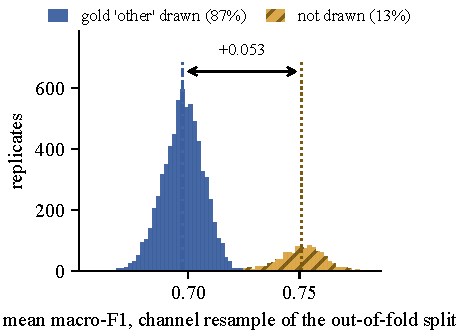
\includegraphics[width=\columnwidth]{fig/divisor.pdf}
\caption{Bootstrap distribution of the system's reported mean macro-F1 over $8{,}000$ channel
resamples of the out-of-fold split (\S\ref{sec:divisor}). The predictions are identical in
every replicate. The separation is due entirely to whether the resample contains one of the two
gold \lab{other} rows, which changes the ST1 average from five classes to four.}
\label{fig:divisor}
\end{figure}

\paragraph{Code.}
All measurements in this paper are produced by scripts in the repository at
\url{https://github.com/thylinao1/childsafeads}: \lab{clinic/presence\_artefact.py}
(\S\ref{sec:divisor}), \lab{clinic/level\_ablation.py} (Table~\ref{tab:levels}),
\lab{clinic/member\_ablation.py} (Table~\ref{tab:members}),
\lab{clinic/advertiser\_overlap.py} (\S\ref{sec:advertiser}) and
\lab{clinic/hand\_label\_audit.py} (\S\ref{sec:hand}) and \lab{clinic/per\_class\_report.py}
(Table~\ref{tab:perclass}), with the pinned scorer in \lab{eval/local\_scorer.py}, the pipeline
figure in \lab{clinic/make\_pipeline\_figure.py}, and the manifest-checked submission generator
of \S\ref{sec:hand} in \lab{generate\_submission.py} (\lab{--from-manifest}).

\section{Evaluation findings in detail}
\label{app:evaluation}

\paragraph{Divisor variance (\S\ref{sec:divisor}).}
The two gold \lab{other} rows sit in two of the $632$ out-of-fold channels. With the class
present, ST1 averages over five classes; with it absent, over four, so the ST1 column moves by
$+0.1604$ against a predicted $+0.1590$, a four-class average being exactly $5/4$ of a
five-class one, and the reported mean by $+0.0530$. Three consequences follow. A marginal
standard error is not a sufficient summary of a score on this metric: the marginal figure of
$0.0200$ is roughly twice the within-regime figures ($0.0090$ with the class present, $0.0102$
without), and none of the excess reflects a property of the system. Two rows of a class no system emits outweigh the gap between the two leading
systems. And whether to emit such a class cannot be decided from the training data: firing and
missing costs a false positive, never firing costs the whole class slot, and which is worse
depends on the hidden gold.

\paragraph{Divisor recovery (\S\ref{sec:invert}).}
For the constant predictor, $tp=g$, $fp=N-g$ and $fn=0$, so $\mathrm{F1}(c)=2g/(N+g)$; every
other gold-present class scores $0$ and classes absent from both gold and predictions are
dropped, which gives $S=2g/\bigl(K(N+g)\bigr)$. On the development split the solution $g=218$
back-substitutes to $0.150970$, matching the published $0.1510$, and the development gold has
exactly four of the five ST1 classes. On the evaluation split the two surviving candidates
differ on the point at issue, because $K=5$ requires \lab{other} to be present: $235/503=0.467$
sits on the pooled labelled \lab{physical\_goods} rate of $0.4701$, while $172/503=0.342$ is
more than three standard deviations of a channel-block bootstrap away. The system set
\lab{other} never to fire, reasoning that a class with two training instances is more likely
absent than present; the inversion shows that reasoning to have been wrong. The organisers
confirmed the recovery against their own labels (personal communication).

Recovering labels from leaderboard feedback is established: Blum and Hardt
\shortcite{blum2015ladder} formalise leaderboard overfitting, Whitehill \shortcite{whitehill2016auc}
inverts an AUC oracle, and Aggarwal et al. \shortcite{aggarwal2021label} recover labels from
log-loss scores, a strictly stronger result. Here the channel is passive, the organisers having
published the baseline row themselves; the leak sits in the metric's divisor rather than its
numerator; and four published decimals suffice to invert, a concrete case of the precision
heuristic Blum and Hardt leave open. Fixing the label set for the average removes both the
variance and the inversion in one step, at the cost only of rare classes scoring $0$ by an
explicit rather than an implicit choice; failing that, the baseline can be reported on a split
that is not being scored, at fewer decimals, or as a bootstrapped score
\cite{chaibubneto2016reducing}. The adaptive-analysis literature
\cite{dwork2015reusable,lin2022msmarco} and the case against reading a leaderboard as a ranking
\cite{ethayarajh2020utility} bear on the same problem.

\paragraph{Advertiser overlap (\S\ref{sec:advertiser}).}
No channel is shared between the evaluation split and the labelled data, so the overlap is
entirely at the advertiser level, and because $66.7\%$ of training rows have their advertiser
in another fold, out-of-fold estimates are partly measured on advertisers already fitted. The
lookup assigns ST1 exactly right on $93.0\%$ of the $358$ development rows whose advertiser is
labelled, against $0.7352$ mean macro-F1 for the full system on that split, and its gains over
the majority baseline are $+0.534$ on ST1, $+0.657$ on ST2 and $+0.283$ on ST3; the advertiser
proxy will merge distinct advertisers that share a platform domain and split advertisers across
country domains. A future edition might report an advertiser-disjoint split
alongside the channel-disjoint one.

\section{Per-class results}
\label{app:perclass}

\begin{table}[t]
\centering\footnotesize
\setlength{\tabcolsep}{3pt}
\begin{tabular}{@{}lrrrrrr@{}}
\toprule
& \multicolumn{4}{c}{out-of-fold (2353)} & \multicolumn{2}{c}{dev (504)} \\
\cmidrule(lr){2-5}\cmidrule(l){6-7}
Class & $n$ & P & R & F1 & $n$ & F1 \\
\midrule
\multicolumn{7}{@{}l}{\emph{ST1, macro-F1 0.6369 / 0.8519}} \\
physical goods & 1125 & 0.96 & 0.95 & 0.95 & 218 & 0.93 \\
digital content/services & 1069 & 0.94 & 0.94 & 0.94 & 248 & 0.94 \\
physical services & 122 & 0.76 & 0.72 & 0.74 & 24 & 0.84 \\
none & 35 & 0.46 & 0.69 & 0.55 & 14 & 0.69 \\
other & 2 & -- & 0.00 & 0.00 & 0 & -- \\
\midrule
\multicolumn{7}{@{}l}{\emph{ST2, macro-F1 0.8423 / 0.7572}} \\
toys & 77 & 0.79 & 0.84 & 0.82 & 8 & 0.71 \\
food & 293 & 0.95 & 0.95 & 0.95 & 49 & 0.95 \\
apps & 654 & 0.83 & 0.88 & 0.85 & 171 & 0.86 \\
hardware/electronics & 516 & 0.84 & 0.89 & 0.87 & 120 & 0.91 \\
fashion & 267 & 0.87 & 0.90 & 0.88 & 50 & 0.83 \\
health & 264 & 0.89 & 0.84 & 0.87 & 55 & 0.88 \\
education & 140 & 0.85 & 0.91 & 0.88 & 12 & 0.70 \\
financial & 135 & 0.90 & 0.84 & 0.87 & 20 & 0.74 \\
gambling & 12 & 1.00 & 0.92 & 0.96 & 5 & 0.50 \\
gambling-adjacent & 92 & 0.72 & 0.79 & 0.76 & 17 & 0.78 \\
creator community & 269 & 0.78 & 0.72 & 0.75 & 47 & 0.67 \\
other & 412 & 0.63 & 0.71 & 0.67 & 87 & 0.57 \\
\midrule
\multicolumn{7}{@{}l}{\emph{ST3, macro-F1 0.6199 / 0.5966}} \\
undisclosed advertising & 352 & 0.87 & 0.86 & 0.87 & 74 & 0.84 \\
inadequate disclosure & 611 & 0.48 & 0.61 & 0.54 & 118 & 0.45 \\
direct exhortation & 304 & 0.45 & 0.56 & 0.50 & 77 & 0.54 \\
misleading claim & 1277 & 0.74 & 0.81 & 0.78 & 260 & 0.78 \\
age-restricted product & 59 & 0.66 & 0.69 & 0.68 & 16 & 0.69 \\
HFSS food marketing & 40 & 0.42 & 0.70 & 0.52 & 5 & 0.26 \\
no flag & 529 & 0.57 & 0.60 & 0.58 & 127 & 0.54 \\
insufficient context & 15 & 0.54 & 0.47 & 0.50 & 7 & 0.67 \\
\bottomrule
\end{tabular}
\caption{Per-class results of the system on the two labelled splits under the present-label
convention: gold count $n$, precision, recall and F1 out of fold, and gold count and F1 on
dev. A class absent from both gold and predictions is dropped from the average (dashes).}
\label{tab:perclass}
\end{table}

\begin{table}[t]
\centering\footnotesize
\setlength{\tabcolsep}{4pt}
\begin{tabular}{@{}lrrrrr@{}}
\toprule
gold $\backslash$ predicted & PG & DC & PS & N & O \\
\midrule
PG (physical goods) & 1064 & 38 & 15 & 8 & 0 \\
DC (digital content/services) & 32 & 1009 & 11 & 17 & 0 \\
PS (physical services) & 8 & 23 & 88 & 3 & 0 \\
N (none) & 5 & 4 & 2 & 24 & 0 \\
O (other) & 1 & 1 & 0 & 0 & 0 \\
\bottomrule
\end{tabular}
\caption{ST1 confusion matrix on the out-of-fold split, gold in rows and predictions in
columns.}
\label{tab:confusion}
\end{table}

Tables~\ref{tab:perclass} and \ref{tab:confusion} are produced by
\lab{clinic/per\_class\_report.py} from the canonical emission scored in
Table~\ref{tab:results}.

\end{document}
